% 第 4 章续：拓扑互连规划
\section{执行拓扑互连规划}
\subsection*{Performing Topology Interconnect Planning}

可以用拓扑互连规划（topology interconnect planning）方法，为大量总线信号定义并创建布线拓扑。

\begin{seeAlsoBox}
更多说明见 \emph{IC Compiler II Design Planning User Guide} 中的 Topology Interconnect Planning。
\end{seeAlsoBox}

在拓扑互连规划流程中，统一拓扑约束（unified topology constraint，UTC）为版图中总线信号的布线拓扑提供一种共同的约束语言和方法。UTC 的基本构成是拓扑规划（topology plan）、拓扑节点（topology node）、拓扑边（topology edge）和拓扑中继器（topology repeater）。

下列各节说明可以在 GUI 中对这些构件执行的部分操作。
\begin{itemize}
  \item 使用 Topology Toolbox
  \item 使用 Create Topology Layout 工具
  \item 用定制符号表示拓扑节点
  \item 使用 Move Topology Object 工具
  \item 把拓扑节点附着到有效的重叠对象
  \item 把拓扑节点连成菊花链
  \item 设置拓扑边的形状层
  \item 使用拓扑组与拓扑规划
  \item 使用束对象
  \item 在 GUI 中查看拓扑时序估算结果
\end{itemize}

\subsection{使用 Topology Toolbox}
\subsubsection*{Using the Topology Toolbox}

可以从 Topology Toolbox（\textbf{View > Toolbars > Topology Toolbox} 或 \textbf{View > Assistants > Topology Toolbox}）访问全部与拓扑互连规划相关的命令和实用功能。

\begin{longtable}{@{}>{\raggedright\arraybackslash}p{0.16\textwidth}>{\raggedright\arraybackslash}p{0.24\textwidth}>{\raggedright\arraybackslash}p{0.54\textwidth}@{}}
\caption{Topology Toolbox}\label{tab:gui-dp-toolbox}\\
\toprule
区段 & 工具界面 & 说明 \\
\midrule
\endfirsthead
\caption*{表~\thetable{}（续）：Topology Toolbox}\\
\toprule
区段 & 工具界面 & 说明 \\
\midrule
\endhead
\bottomrule
\endlastfoot
工具栏（Toolbar） & 下列按钮 &
\textbullet\ Design Assistant：执行设计规划任务\newline
\textbullet\ Create Topology Layout：创建节点、边、中继器等拓扑对象\newline
\textbullet\ Lock：把所选对象锁定在当前位置以便编辑\newline
\textbullet\ Unlock：解除所选对象的锁定\newline
\textbullet\ Set topology objects visible：把拓扑对象设为可见\newline
\textbullet\ Set topology objects invisible：把拓扑对象设为不可见\newline
\textbullet\ Set net estimation rule：设置线网估算规则\newline
\textbullet\ Associate selected annotation shapes with topology plan：把所选或当前拓扑规划与所选标注形状（annotation shape）关联。若选择了不止一个拓扑规划，该操作被禁用。把标注形状与拓扑规划关联之后，其可见性由所关联拓扑规划的可见性决定，并同时受 View Settings 面板中标注形状可见性设置的影响。 \\
\addlinespace
规划（Plan） & 下列按钮 &
\textbullet\ Create：创建拓扑规划\newline
\textbullet\ Characterize：特征化（characterize）拓扑规划\newline
\textbullet\ Create Default：创建默认拓扑规划\newline
\textbullet\ Refine：细化（refine）拓扑规划\newline
\textbullet\ Create Group：创建拓扑组\newline
\textbullet\ Uniquify：唯一化（uniquify）拓扑规划\newline
\textbullet\ Optimize：优化拓扑规划\newline
\textbullet\ Write：写出拓扑规划 \\
\addlinespace
选择（Select） & 用于下列操作的按钮 &
\textbullet\ 选择相关拓扑规划\newline
\textbullet\ 选择相关拓扑边\newline
\textbullet\ 选择相关拓扑节点\newline
\textbullet\ 选择相关拓扑中继器\newline
\textbullet\ 选择相连的拓扑 \\
\addlinespace
编辑（Edit） & 用于下列操作的按钮 &
\textbullet\ 移动或附着拓扑对象\newline
\textbullet\ 合并拓扑节点\newline
\textbullet\ 删除所选拓扑节点\newline
\textbullet\ 把有效的重叠对象与所选拓扑节点关联\newline
\textbullet\ 删除与拓扑规划关联的布线 \\
\addlinespace
边（Edge） & 用于下列操作的按钮 &
\textbullet\ 用不同选项自动循环形状。循环顺序：Auto $\rightarrow$ L-Shape (x) $\rightarrow$ L-Shape (y) $\rightarrow$ S-Shape (x) $\rightarrow$ S-Shape (y)\newline
\textbullet\ 自动设置边的形状\newline
\textbullet\ Set edge L-Shape (X-First)，即先水平\newline
\textbullet\ Set edge L-Shape (Y-First)，即先垂直\newline
\textbullet\ Set edge S-Shape (X-First)\newline
\textbullet\ Set edge S-Shape (Y-First)\newline
\textbullet\ 反转边的方向\newline
\textbullet\ 按线网估算规则设置边的层\newline
\textbullet\ 估算拓扑边\newline
\textbullet\ 重置拓扑边估算，即把边形状的宽度重置为零 \\
\addlinespace
连接（Connection） & 用于下列操作的按钮 &
\textbullet\ 创建鱼骨连接（fishbone connection）\newline
\textbullet\ 创建链式连接（chain connection）\newline
\textbullet\ 创建星形连接（star connection）\newline
\textbullet\ 向左连接节点\newline
\textbullet\ 向右连接节点\newline
\textbullet\ 向上连接节点\newline
\textbullet\ 向下连接节点 \\
\addlinespace
分析（Analyze） & 用于下列操作的按钮 &
\textbullet\ 检查拓扑规划\newline
\textbullet\ 估算拓扑规划 \\
\addlinespace
实现（Implement） & 用于下列操作的按钮 &
\textbullet\ 创建拓扑干线（trunk）\newline
\textbullet\ 实现拓扑中继器\newline
\textbullet\ 删除与拓扑规划关联的布线\newline
\textbullet\ 删除所选拓扑规划上已放置和已创建的中继器 \\
\end{longtable}

\subsubsection{定制 Topology Toolbox}
\subsubsection*{Customizing the Topology Toolbox}

要把常用操作加入 Topology Toolbox，可以定制该工具箱，并把操作加到一个新的 User 区。

下面的示例向 Topology Toolbox 加入两个按钮 Nudge Left 与 Nudge Right，使视图略向左和向右平移。
\begin{lstlisting}
gui_create_menu -menu "My_Menu->&Nudge_Right" \
   -tcl_cmd {gui_scroll \
   -window [gui_get_current_window -view] -hrel .05}
gui_create_menu -menu "My_Menu->&Nudge_Left" \
   -tcl_cmd {gui_scroll \
   -window [gui_get_current_window -view] -hrel -.05}
gui_set_pref_value -category topologyToolbox \
   -key userButtonsList -value "My_Menu->Nudge_Right My_Menu->Nudge_Left"
\end{lstlisting}

\subsection{使用 Create Topology Layout 工具}
\subsubsection*{Using the Create Topology Layout Tool}

要创建节点、边、中继器等拓扑对象，使用 Create Topology Layout 工具。也可以为形状层创建带混合值（百分比与距离）的拓扑边。

用该工具定义凸点区域（bump region）之间的连接，以建立芯片到芯片的连接。也可以像对待任何其他有效对象一样，用 \cmd{create\_topology\_node} 命令把拓扑节点与凸点区域关联；可在 Create Topology Layout 工具、Move Topology Object 工具中执行，或通过 Properties Editor 执行。

可以按下列方式使用拓扑版图工具：
\begin{enumerate}
  \item 在 \textbf{Design Assistant > Topologies} 选项卡中选择一个拓扑规划。
  \item 用下列方法之一打开 Create Topology Layout 工具栏：
  \begin{itemize}
    \item 在 \textbf{Design Assistant > Topologies} 选项卡中选择 \textbf{Create > Topology Layout}。
    \item 在 \textbf{Design Assistant > Topologies} 选项卡中，右键单击拓扑规划，再单击 Topology Layout。
    \item 在块窗口中选择 \textbf{Create > Topology Layout}。
  \end{itemize}
\end{enumerate}

\begin{figure}[htbp]
\centering
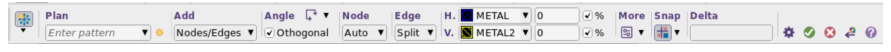
\includegraphics[width=0.92\textwidth]{gui-fig-074.png}
\caption{创建拓扑版图工具栏}
\label{fig:gui-74}
\end{figure}

\begin{enumerate}
  \setcounter{enumi}{2}
  \item 在版图视图中，单击要连接的拓扑节点对象，或从新的拓扑节点开始。
  \item 把光标移到下一个目标，它可以是已有的或新的拓扑节点。移动指针时，工具只勾勒出可以与新节点关联的对象。
  \item 单击鼠标按钮以放置节点。
  \item 单击末端对象（拓扑节点）以完成布线，或双击以用新节点结束。
\end{enumerate}

要把选项重置为默认值，使用 Create Topology Layout 工具栏上的相应图标（见图~\ref{fig:gui-74}）。

要撤销所做的更改，选择 \textbf{Edit > Undo}。

\begin{longtable}{@{}>{\raggedright\arraybackslash}p{0.32\textwidth}>{\raggedright\arraybackslash}p{0.64\textwidth}@{}}
\caption{Create Topology Layout 工具选项}\label{tab:gui-dp-layout}\\
\toprule
选项 & 说明 \\
\midrule
\endfirsthead
\caption*{表~\thetable{}（续）：Create Topology Layout 工具选项}\\
\toprule
选项 & 说明 \\
\midrule
\endhead
\bottomrule
\endlastfoot
Plan & 指定新节点、边和中继器所加入的拓扑规划名称。创建拓扑规划。 \\
\addlinespace
Add & 指定要添加的对象类型。 \\
\addlinespace
Angle & 在正交输入模式（orthogonal input mode）下设置起始输入方向。 \\
\addlinespace
Orthogonal & 切换正交输入方向。 \\
\addlinespace
Node & 指定拓扑节点的节点约束类型。 \\
\addlinespace
Edge & 设为 Split 时，在拓扑边中点插入新节点，把最后一条边拆成两条；否则创建抽头节点（tap node）。 \\
\addlinespace
Horizontal Layer/Width/Length Percentage & 指定水平边的形状层与宽度。选中水平长度百分比选项时，工具按百分比设置水平边形状长度；否则边长设为绝对长度。 \\
\addlinespace
Vertical Layer/Width/Length Percentage & 指定垂直边的形状层与宽度。选中垂直长度百分比选项时，工具按百分比设置垂直边形状长度；否则边长设为绝对长度。 \\
\addlinespace
Snap & 打开或关闭把拓扑节点吸附（snap）到可见或可选对象。 \\
\addlinespace
Delta & 为版图编辑输入点时，指定相对活动推断点（inference point）的偏移信息。 \\
\addlinespace
More > Node > Attach & 设为 true 时，预选并标注该节点可以附着的有效对象。 \\
\addlinespace
More > Node > Prefer pins & 设为 true 时，把拓扑节点与管脚关联，而不是与块关联。 \\
\addlinespace
More > Node > Routing target & 指定约束类型为 edge、side 和 bounding box 的节点能否作为布线目标。 \\
\addlinespace
More > Actions > Auto apply & 设为 true 时，新节点（边的末端节点）关联到任何有效对象（块、管脚、端口等）后即结束输入。 \\
\addlinespace
More > Show > Port Guidance & 显示管脚连接与位置的引导。 \\
\addlinespace
More > Show > Flylines & 显示指定线网的管脚飞线（flyline），或到最近开口（open）的飞线。 \\
\addlinespace
More > Show > Routes & 高亮指定的线网或束。 \\
\end{longtable}

\subsection{用定制符号表示拓扑节点}
\subsubsection*{Using Custom Symbols to Represent Topology Nodes}

默认情况下，工具用下列约定表示拓扑节点。

\begin{table}[htbp]
\centering
\caption{拓扑节点的默认符号}
\label{tab:gui-dp-nodesym}
\begin{tabularx}{\textwidth}{@{}l X@{}}
\toprule
拓扑节点 & 符号 \\
\midrule
起始节点（start node） & 圆（circle） \\
中间节点（intermediate node） & 菱形（diamond） \\
结束节点（end node） & 正方形（square） \\
\bottomrule
\end{tabularx}
\end{table}

需要时，可以用定制符号表示这些节点。要使用定制符号：
\begin{enumerate}
  \item 在 Layout View 中选择该节点。
  \item 打开 Properties Editor。
  \item 切换到 Application 属性组。
  \item 从 symbol 下拉列表中选择一种符号。
  \item 单击 Apply Changes。
\end{enumerate}

\subsection{使用 Move Topology Object 工具}
\subsubsection*{Using the Move Topology Object Tool}
\label{sec:gui-dp-move}

要移动拓扑节点，以及把拓扑节点与允许的对象关联或解除关联，使用 Move Topology Object 工具。若要同时自动关联许多拓扑节点，见第~\ref{sec:gui-dp-attach}~节。

\begin{figure}[htbp]
\centering
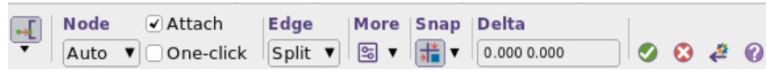
\includegraphics[width=0.92\textwidth]{gui-fig-075.png}
\caption{移动拓扑对象工具栏}
\label{fig:gui-75}
\end{figure}

流程如下：
\begin{enumerate}
  \item 选择 \textbf{Edit > Topology > Move}。
  \item 单击要修改的拓扑节点。
  \item 把节点移到新位置。
\end{enumerate}

要把选项重置为默认值，使用 Move Topology Object 工具栏上的相应图标（见图~\ref{fig:gui-75}）。

要撤销所做的更改，选择 \textbf{Edit > Undo}。

Move Topology Object 工具栏上的 Node、Edge、More、Snap 和 Delta 选项，与 Create Topology Layout 工具栏上的对应选项行为相同。详见第~\ref{tab:gui-dp-layout}~表。

要让拓扑边的形状层使用层颜色，或为起始、中间和结束拓扑节点使用不同颜色，按图~\ref{fig:gui-76} 所示使用相应选项。

\begin{figure}[htbp]
\centering
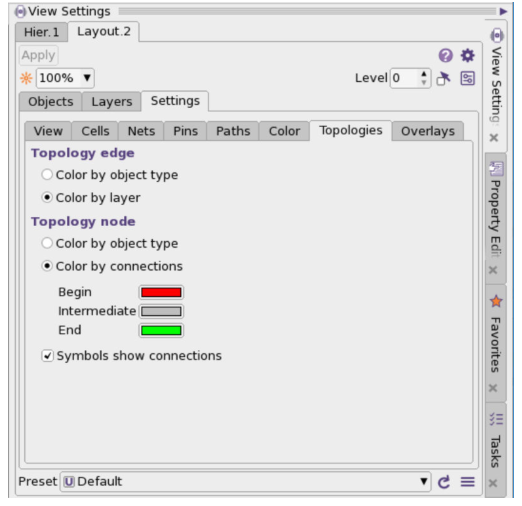
\includegraphics[width=0.92\textwidth]{gui-fig-076.png}
\caption{为拓扑边与拓扑节点使用着色}
\label{fig:gui-76}
\end{figure}

\subsection{把拓扑节点附着到有效的重叠对象}
\subsubsection*{Attaching Topology Nodes With Valid Overlapped Objects}
\label{sec:gui-dp-attach}

在把拓扑规划或边复制或移动到目标位置时，要自动把拓扑节点附着到与这些节点重叠的有效对象，使用 \cmd{attach\_topology\_nodes} 命令。若要逐个附着拓扑节点，使用 Move Topology Object 工具（详见第~\ref{sec:gui-dp-move}~节）。

有效的重叠对象包括：
\begin{itemize}
  \item 标注形状（annotation shape）
  \item 约束（bound）
  \item 约束形状（bound shape）
  \item 凸点区域（bump region）
  \item 单元（cell）
  \item 管脚（pin）
  \item 端口（port）
  \item 形状（shape）
  \item 布局阻塞（placement blockage）
  \item 布线阻塞（routing blockage）
  \item 拓扑边（topology edge）
  \item 端子（terminal）
  \item 电压区域（voltage area）
  \item 电压区域形状（voltage area shape）
\end{itemize}

存在许多重叠对象时，管脚和端口的优先级高于单元，单元的优先级高于其他类型的对象。

在下面的示例中，工具尝试把拓扑规划 tp1 中的全部拓扑节点附着到有效对象。
\begin{lstlisting}
icc2_shell> attach_topology_nodes [get_topology_nodes \
   -of_objects [get_topology_plans tp1]]
\end{lstlisting}

\begin{seeAlsoBox}
更多说明见 \cmd{attach\_topology\_nodes} 命令的 man 页。
\end{seeAlsoBox}

\subsection{把拓扑节点连成菊花链}
\subsubsection*{Daisy Chaining Topology Nodes}

要在当前块中按给定方向快速连接所选或指定的拓扑节点，即把它们连成菊花链（daisy chain）：
\begin{enumerate}
  \item 在版图视图中选择要连接的拓扑节点。
  \item 在指定方向上于所选节点之间创建拓扑边：选择 \textbf{Edit > Topology > Connect Nodes Down}（Up、Left、Right）。
\end{enumerate}

也可以使用相应的上下文相关菜单命令，或 \cmd{connect\_topology\_nodes} 命令。

\begin{noteBox}
若某些节点已经相连，它们会被排除在该操作之外。
\end{noteBox}

\begin{table}[htbp]
\centering
\caption{连接拓扑节点}
\label{tab:gui-dp-connect}
\begin{tabularx}{\textwidth}{@{}XXXX@{}}
\toprule
向下连接拓扑节点 & 向上连接拓扑节点 & 向左连接拓扑节点 & 向右连接拓扑节点 \\
\midrule
版图示意 & 版图示意 & 版图示意 & 版图示意 \\
\bottomrule
\end{tabularx}
\end{table}

\subsection{设置拓扑边的形状层}
\subsubsection*{Setting Topology Edge Shape Layers}

本工具可以为所选或指定的拓扑边设置形状层，或反转其方向。
\begin{enumerate}
  \item 在版图视图中，选择需要设置形状层的拓扑边。
  \item 选择 \textbf{Edit > Topology}，再执行下列操作之一：
\end{enumerate}

\begin{table}[htbp]
\centering
\caption{为拓扑边设置形状层}
\label{tab:gui-dp-shapelayer}
\begin{tabularx}{\textwidth}{@{}X l@{}}
\toprule
要执行的操作 & 使用此功能 \\
\midrule
第一段沿 x 方向的 L 形 & Set Edge L-Shape (X First) \\
第一段沿 y 方向的 L 形 & Set Edge L-Shape (Y First) \\
第一段沿 x 方向的 S 形 & Set Edge S-Shape (X First) \\
第一段沿 y 方向的 S 形 & Set Edge S-Shape (Y First) \\
按起始与结束拓扑节点的接入方向自动选择形状模板 & Set Topology Edge Auto \\
交换起始节点与结束节点，从而反转边的方向 & Reverse Topology Edge Direction \\
按线网估算规则的层定义更新边的形状层 & Set Edge NER Layers \\
\bottomrule
\end{tabularx}
\end{table}

\subsection{使用拓扑组与拓扑规划}
\subsubsection*{Working With Topology Groups and Topology Plans}

\begin{itemize}
  \item 设置当前拓扑组
  \item 删除拓扑组
  \item 查看并编辑拓扑组的聚合属性
  \item 唯一化拓扑规划
  \item 自动选择拓扑规划
  \item 合并堆叠的拓扑节点
\end{itemize}

拓扑组可以把拓扑规划分成多个更小的组。随后可以独立处理这些较小的部分，从而把大型设计分成可管理的部分。它也可以把相似的拓扑规划分在一组，以便对一组拓扑规划执行修改、删除等操作。

流程如下：
\begin{enumerate}
  \item 创建线网估算规则（net estimation rule）。

  线网估算规则定义布线层、非默认布线规则（nondefault routing rule）、中继器单元名、中继器单元间距、时钟，以及其他与布线和时序相关的约束。创建拓扑规划之后，把一条线网估算规则与该拓扑规划关联。需要时，可以从 Properties Editor 面板、Design Assistant，或从自动生成的命令表单（例如 \cmd{create\_topology\_plan} 命令对话框）为一条拓扑规划或一条拓扑边关联多条线网估算规则。
  \begin{enumerate}[label=\alph*.]
    \item 选择 \textbf{View > Assistants > Design Assistant}，打开 Design Assistant。
    \item 选择 \textbf{Create > Net Estimation Rule}。
    \item 按需要在 \cmd{set\_net\_estimation\_rule} 对话框中输入信息，再单击 OK。
  \end{enumerate}

  也可以用 Design Assistant 的 TopologyPlans 与 TopologyGroups 选项卡上的上下文相关菜单创建线网估算规则（在拓扑规划或拓扑组上右键单击，再从菜单选择 Create Net Estimation Rule）。

  \begin{seeAlsoBox}
  关于为拓扑规划创建线网估算规则的更多说明，见 \emph{IC Compiler II Design Planning User Guide} 中的 Creating Net Estimation Rules for Topology Plans。
  \end{seeAlsoBox}

  \item 为线网创建拓扑规划。
  \begin{enumerate}[label=\alph*.]
    \item 单击 Nets 选项卡，用 \cmd{get\_nets} 命令填充列表。
    \item 从列表中选择线网，右键单击所选内容，再选择 Create Topology Plan。
    \item 按需要在 \cmd{create\_topology\_plan} 对话框中输入信息，再单击 OK。
    \item 选择 \textbf{View > New topology Plans}，打开 TopologyPlans 选项卡。
    \item 在 TopologyPlans 选项卡上，用 \cmd{get\_topology\_plans} 命令查看新创建的拓扑规划。
    \item 按需要创建足够多的拓扑规划。
  \end{enumerate}

  创建时，全部拓扑规划都被分配到默认拓扑组 \cmd{DEFAULT\_TOPOLOGY\_GROUP}。group 列显示该拓扑规划所关联的拓扑组。也可以在拓扑规划上右键单击，并从上下文相关菜单选择 Get Topology Group，查看它所属的拓扑组。

  用下列步骤把拓扑规划重新分配到指定的拓扑组。

  \item 为特定拓扑规划创建拓扑组。
  \begin{enumerate}[label=\alph*.]
    \item 在 TopologyPlans 选项卡上，从列表中选择拓扑规划，右键单击所选内容，再选择 Create Topology Group。

    一个拓扑规划只属于一个拓扑组。不能在多个拓扑组之间共享拓扑规划。
    \item 按需要在 \cmd{create\_topology\_group} 对话框中输入信息，再单击 OK。
  \end{enumerate}

  若为拓扑组指定了名称，且当前块中已存在该名称，工具会报错。不过，设计的不同块中可以有同名的拓扑组。若不为拓扑组指定名称，工具自动分配格式为 \cmd{TOPOLOGY\_GROUP<\#n>} 的名称，其中 n 是从 1 开始的整数。

  \begin{noteBox}
  若一个拓扑组包含多个规划，且这些规划在某个属性上的值不同，工具把该属性的值显示为 \cmd{<mixed>}。例如，拓扑组 TG1 有两个拓扑规划 TP1 与 TP2，颜色分别为红色和蓝色，则在 TopologiesGroup 选项卡中，颜色列显示 \cmd{<mixed>}。

  可以把显示为 \cmd{<mixed>} 的值更新为符合要求的值。但不能把属性设为 \cmd{<mixed>}。若提供的值对该属性无效，工具会报错。
  \end{noteBox}

  \begin{seeAlsoBox}
  关于创建拓扑组的更多说明，见 \emph{IC Compiler II Design Planning User Guide} 中的 Creating Topology Groups。
  \end{seeAlsoBox}
\end{enumerate}

把拓扑规划与拓扑组关联之后，可以在 TopologyPlans 选项卡的 group 列中查看这一关联。

要处理一组特定的拓扑规划：
\begin{enumerate}
  \item 在 TopologiesGroups 选项卡上，选择相关的拓扑组。

  若创建拓扑组时添加了注释，可以用 comment 列中的这一信息挑选相关拓扑组。
  \item 右键单击所选拓扑组，并选择 Get Topology Plans。
\end{enumerate}

属于该拓扑组的拓扑规划显示在 TopologiesPlans 选项卡上。可以从 GUI 中提供的选项对这些拓扑规划执行必要操作。

要查看特定拓扑组中的拓扑规划：
\begin{enumerate}
  \item 在 TopologiesGroups 选项卡上，选择拓扑组。
  \item 选择 \textbf{View > Toolbars > Constraints Editor}。
\end{enumerate}

这一步打开 Constraints Editor 视图，列出属于所选拓扑组的全部拓扑规划，以及它们的拓扑节点和边。

\subsubsection{设置当前拓扑组}
\subsubsection*{Setting the Current Topology Group}

创建拓扑组时，它成为当前拓扑组。

要把某个拓扑组设为当前拓扑组：
\begin{enumerate}
  \item 在 TopologiesGroups 选项卡上，选择相关的拓扑组。
  \item 选择 \textbf{Edit > Topology > Set Current Group}，或在 Design Assistant 的上下文菜单中选择 Set Current Topology Group。
\end{enumerate}

\begin{seeAlsoBox}
关于创建拓扑组的更多说明，见 \emph{IC Compiler II Design Planning User Guide} 中的 Setting the Current Topology Group。
\end{seeAlsoBox}

\subsubsection{删除拓扑组}
\subsubsection*{Removing Topology Groups}

不再需要一个或多个拓扑组时，可以选择这些拓扑组，再选择 \textbf{Edit > Topology > Remove Group} 菜单，从 GUI 中删除它们。删除含有拓扑规划的拓扑组时，工具自动把这些拓扑规划移到默认拓扑组。若默认拓扑组中还有任何拓扑规划，则不能删除默认拓扑组；不过可以对 \cmd{remove\_topology\_groups} 命令使用 \opt{-remove\_plans} 选项，同时删除拓扑规划和默认拓扑组。

\begin{seeAlsoBox}
关于创建拓扑组的更多说明，见 \emph{IC Compiler II Design Planning User Guide} 中的 Removing Topology Groups。
\end{seeAlsoBox}

\subsubsection{查看并编辑拓扑组的聚合属性}
\subsubsection*{Viewing and Editing Aggregate Attributes of Topology Groups}

IC Compiler II 工具支持编辑拓扑组的聚合属性。

当拓扑组中不同拓扑规划在某个属性上的值不同时，工具聚合该属性的值，并把它们显示为一个聚合属性。例如，若拓扑组中拓扑规划 A 与拓扑规划 B 的颜色分别为红色和蓝色，则拓扑组的颜色列对颜色属性显示 \cmd{<mixed>}。

要更改聚合属性的值：
\begin{enumerate}
  \item 选择 \textbf{View > Assistants > Design Assistant}。
  \item 在 TopologyGroups 选项卡上，选择该拓扑组。
  \item 要应用或编辑颜色：
  \begin{enumerate}[label=\alph*.]
    \item 单击颜色列中的调色板图标。
    \item 从 Select Color 对话框中选择一种颜色。
    \item 单击 OK。
  \end{enumerate}

  颜色被应用到所选拓扑组以及与该拓扑组关联的全部拓扑规划。颜色列显示用 Select Color 对话框所选颜色的十六进制值，格式为 24 位 RGB 十六进制字符串，例如 \cmd{\#aa0000}。
  \item 要编辑拓扑组是否可见：
  \begin{enumerate}[label=\alph*.]
    \item 单击 \cmd{is\_visible} 列中的下拉列表。

    把拓扑规划的 \cmd{is\_visible} 属性设为 true 或 false，可以控制在版图视图中查看哪些拓扑规划。拓扑规划很多、又只想每次处理其中少数几个时，该功能很有用。
    \item 把值设为 true 或 false。

    不能把属性值设为 \cmd{<mixed>}。当所选拓扑组中的拓扑规划在 \cmd{is\_visible} 属性上的值不同时，工具自动把该值填为 \cmd{<mixed>}。
    \item 单击 Apply Changes。
  \end{enumerate}
  \item 要编辑所选拓扑组的物理状态（physical status）：
  \begin{enumerate}[label=\alph*.]
    \item 单击 \cmd{physical\_status} 列中的下拉列表。
    \item 把值设为 locked 或 unrestricted。默认值为 unrestricted。

    不能把属性值设为 \cmd{<mixed>}。

    物理状态为 locked 时，可防止对拓扑规划做意外的物理编辑（移动、拉伸等）。拓扑规划的各个要素（节点、边和中继器）也有 locked 与 unrestricted 状态。要编辑拓扑节点、边和中继器，它们自身的物理状态以及父拓扑规划的物理状态都必须是 unrestricted（未锁定）。
    \item 单击 Apply Changes。
  \end{enumerate}
\end{enumerate}

\subsubsection{唯一化拓扑规划}
\subsubsection*{Uniquifying Topology Plans}

可以用 \cmd{uniquify\_topology\_plans} 命令，为指定拓扑规划中每一组物理上相连的拓扑节点创建新的拓扑规划。

在下面的示例中，工具把当前拓扑规划拆成连通分量。
\begin{lstlisting}
icc2_shell> uniquify_topology_plans [current_topology_plan]
\end{lstlisting}

除拓扑规划名称外，还可以在 \cmd{uniquify\_topology\_plans} 命令中指定模式和集合。

\begin{seeAlsoBox}
更多说明见该命令的 man 页。
\end{seeAlsoBox}

示例结果中出现下列拓扑规划名称（原稿此处为无图号的示意，文本顺序如下）：
\begin{itemize}
  \item Topology Plan 3
  \item Topology Plan 2
  \item Topology Plan 1
  \item Default topology plan
\end{itemize}

\subsubsection{自动选择拓扑规划}
\subsubsection*{Automatically Select Topology Plans}

对于需要拓扑规划的操作，可以先选择一条拓扑边、一个节点或一个中继器，再继续该操作。随后，操作或命令窗口会自动填入与所选对象关联的拓扑规划。

对于下列操作，关联的拓扑规划会被填入各自的命令窗口：
\begin{itemize}
  \item 特征化规划（Characterize plan）
  \item 检查规划（Check plan）
  \item 估算时序（Estimate timing）
  \item 实现中继器（Implement repeaters）
  \item 实现干线（Implement trunks）
  \item 优化（Optimize）
  \item 唯一化（Uniquify）
  \item 写出（Write）
\end{itemize}

\subsubsection{合并堆叠的拓扑节点}
\subsubsection*{Merging Stacked Topology Nodes}

可以用 \cmd{merge\_objects} 命令合并彼此堆叠的拓扑节点。合并操作有助于去掉多余的拓扑节点。下列命令合并全部所选对象。
\begin{lstlisting}
icc2_shell> merge_objects [get_selection]
\end{lstlisting}

也可以用 GUI（\textbf{Edit > Merge Shapes}）合并所选对象。

\subsection{使用束对象}
\subsubsection*{Working With Bundle Objects}

从工具 GUI（Manage Bundle 对话框，\textbf{Create > Bundle}）可以：
\begin{itemize}
  \item 创建束
  \item 向已有束添加对象
  \item 从已有束中删除对象
  \item 按总线限定符（bus limiter）对总线排序
\end{itemize}

对 n[1] 与 n[2]，总线分隔符是 []。

\subsubsection{创建束}
\subsubsection*{Creating a Bundle}

可以用下列方式之一，用指定线网创建束：
\begin{itemize}
  \item 在块窗口中选择 \textbf{Create > Bundle}
  \item 在 Design Assistant 中选择 \textbf{Create > Bundle}
\end{itemize}

在 Manage Bundle 对话框中：
\begin{enumerate}
  \item 在 Bundle name 字段中输入束的名称，或从下拉列表中选择一个束。

  若在为束命名，须保证束名唯一。
  \item 添加或修改线网列表：
  \begin{itemize}
    \item 通过搜索特定线网：Search
    \item 使用所选版图形状（例如管脚、端子、连线和通孔）的位置：Get selection

    用该选项插入连接到所选对象的线网。工具按对应线网对象的几何形状排列线网。默认顺序是从左到右。要使用不同顺序，在 Get selection 按钮右侧的菜单上选择一条命令。
    \item 加载包含线网名列表的文本文件：Load from file

    在 Read nets from file 资源管理器对话框中选择文件。
    \item 可以对所选线网执行表~\ref{tab:gui-dp-bundle} 中的操作。
  \end{itemize}
  \item 单击 OK 以应用并关闭对话框，或单击 Apply 以继续工作。
\end{enumerate}

\begin{table}[htbp]
\centering
\caption{Manage Bundle 对话框中对所选线网的操作}
\label{tab:gui-dp-bundle}
\begin{tabularx}{\textwidth}{@{}X l@{}}
\toprule
要执行的操作 & 使用此方法 \\
\midrule
对线网排序。排序前，先用 Sort mode、Precedence、Bus delimiter 与 Wildcard list 设置排序首选项。Precedence 选择 Left 时，线网按第一个下标排序；选择 Right 时，线网按最后一个下标排序。更多说明见工具 GUI 中的上下文相关在线帮助。 & Sort \\
\addlinespace
反转束中线网的顺序 & Reverse \\
\addlinespace
选择要删除的线网 & Remove \\
\addlinespace
从束中删除全部线网 & Remove All \\
\bottomrule
\end{tabularx}
\end{table}

\subsection{在 GUI 中查看拓扑时序估算结果}
\subsubsection*{Viewing Estimate Topology Timing Results in GUI}

可以在工具 GUI 中以用户表的形式查看 \cmd{estimate\_topology\_timing} 命令的结果。

要查看结果：
\begin{enumerate}
  \item 打开顶层设计。
\begin{lstlisting}
icc2_shell> open_block orca:ORCA
\end{lstlisting}
  \item 设置约束映射文件。
\begin{lstlisting}
icc2_shell> set_constraint_mapping_file split/mapfile
\end{lstlisting}
  \item 读入由 \cmd{split\_constraints} 命令创建的顶层约束。
\begin{lstlisting}
icc2_shell> source ./split/ORCA/top.tcl
\end{lstlisting}
  \item 在 Topology Toolbox 中单击 Estimate Timing。
  \item 在 \cmd{gui\_estimate\_topology\_timing} 对话框中设置必要选项，再单击 OK。
\end{enumerate}

用户表视图随即打开，并显示时序估算结果。
